\chapter{Práctica: Aspiradora autónoma}\label{cap.roomba}
En este capítulo se expondrá el desarrollo de una nueva práctica para la plataforma de JdeRobot-Academy, que se llama ``Aspiradora autónoma''. En este capítulo se aborda el desarrollo de su infraestructura, su componente académico correspondiente, una gráfica de la derivada del porcentaje, así como el evaluador automático creado y la solución de referencia llevada a cabo. 

\section{Enunciado de la práctica} \label{sec.enunciado}
El objetivo de esta práctica es que una aspiradora robótica sea capaz de limpiar de forma autónoma la mayor superficie posible en una casa. La aspiradora no tendrá ninguna forma de obtener su posición absoluta en el mundo, ya que esa es la situación en los modelos
de gama media y baja existentes en el mercado de electrodomésticos robóticos. El único dato que conocerá la aspiradora es su orientación (fácilmente disponible en modelos reales con una brújula). Además, esta aspiradora posee un sensor láser, que le permite medir la distancia a la que se sitúan los obstáculos. Esta aspiradora tiene un actuador de movimiento que permite controlar su velocidad lineal y velocidad de giro. Todos estos elementos permiten realizar un algoritmo de pilotaje similar al que materializan las aspiradoras robóticas disponibles en el mercado.\\

En esta práctica el alumno deberá programar el algoritmo capaz de limpiar un gran porcentaje de la casa sin autolocalización. En la interfaz gráfica del componente académico se puede visualizar un mapa de la casa, así como la posición de la aspiradora en el mapa y los lugares por donde ha pasado. Este mapa no estará disponible para el algortimo de control, únicamente se utiliza como visualización para el alumno y medida de resultados.  \\

El algoritmo responde a un control reactivo, que en cada instante actuará en función de los datos de los sensores y sus propias variables internas. El control reactivo permitirá controlar en todo momento el movimiento del robot y responder ante situaciones imprevistas.

\section{Infraestructura}
En este apartado se describirá el entorno creado para realizar la práctica ``Aspiradora autónoma''. Además, se describirá el robot que se ha utilizado en esta práctica, sus sensores y actuadores, su modelo dentro del simulador Gazebo, así como el entorno(una casa típica con varias habitaciones, comedor, mesas, sillas,puertas, etc) por el que se mueve este robot. 

\subsection{Roomba}
El robot que se ha empleado en esta práctica es el robot Roomba de la serie 500, que fue comercializado por la empresa iRobot (en Estados Unidos). Esta aspiradora robótica está equipada con un conjunto de sensores con los que explorar sus alrededores y unos actuadores que le permiten moverse adecuadamente por su entorno. Los modelos de Roomba de esta serie poseen sensores infrarrojos, un sensor detector de suciedad, un sensor detector de desniveles, y cuentan además con un bumper.\\

En el caso de la práctica, se empleó el modelo de Roomba de JdeRobot, que no tiene detector de desniveles debido a que el escenario de nuestra práctica no los contiene (no hay escaleras); y tampoco tiene detector de suciedad, puesto que no se ha simulado la suciedad, ya que el objetivo de la práctica era hacer énfasis en el algoritmo de navegación. En nuestro modelo de Roomba tenemos un sensor bumper, que permite detectar los choques con objetos; y un sensor láser, que permite medir la distancia a los objetos. Este sensor láser es capaz de hacer un barrido de 180 grados, con precisión de 1 grado. Además, este robot posee sensores \acrshort{gps}, los cuales le permiten conocer la posición en la que se encuentra el robot en cada momento (la posición no se usará en la solución de referencia, a propósito).\\

El robot Roomba de la serie 500 posee una anchura de 340 milímetros, 92 milímetros de altura, y un peso de 3.6 kg. El modelo Roomba de JdeRobot mide aproximadamente 330 mm de ancho, 90 mm de altura, y un peso de 2.5 kg.\\

\begin{figure}[H]
  \begin{center}
    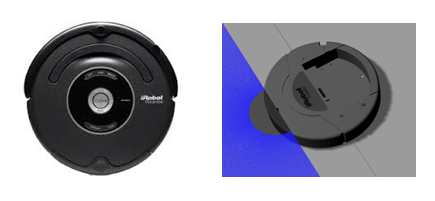
\includegraphics[width=0.6\textwidth]{figures/Vacuum/Roombas.png}
		\caption{Roomba de iRobot y modelo Roomba en Gazebo}
		\label{fig.roombas}
		\end{center}
\end{figure}

En esta práctica se han utilizado cuatro drivers: 

\begin{itemize}
\item pose3di: Los componentes harán uso de este plugin para obtener su posición en tiempo real. Además, este plugin se emplea para modificar la posición de los componentes.
\item motorsi: Este plugin interactúa con el componente, dotándole de velocidad, tanto velocidad de tracción como velocidad de rotación y modifica los datos de la interfaz de usuario.
\item Laseri: Este plugin será usado por los componentes para poder obtener información de la distancia que hay hasta los obstáculos.
\item Bumperi: El componente podrá usar este plugin para recolectar información acerca de su situación de colisión con otro objeto cualquiera.
\end{itemize}

\subsubsection{Sensor láser}
En la parte frontal del robot se ha instalado un sensor láser. Este sensor se utilizará ampliamente en la práctica. Está compuesto por un array de 180 medidas, que puede medir distancia alrededor de 180 grados. Las medidas de distancia que nos devuelve el láser están en milímetros.\\

Una vez más la plataforma JdeRobot encapsula la complejidad de este sensor y nos devuelve los datos que ofrece el mismo, en forma de un array de 180 distancias.

\subsubsection{Sensor bumper}
El sensor bumper es un sensor de contacto que permite detectar una colisión con un objeto. Esto va a ser muy útil para realizar el algoritmo de esta práctica. Este sensor comprueba el número de contactos con obstáculos del entorno, y si dicho número es mayor que cero es porque el robot ha chocado con algún objeto. La plataforma JdeRobot abstrae del funcionamiento interno de este sensor, y permite conocer si ha habido algún choque devolviéndonos un 0 o un 1. Si el robot se ha chocado con algún objeto, entonces el bumper nos devolverá un 1. Por el contrario, si el robot no colisiona con ningún obstáculo, entonces el bumper nos dará como resultado un 0.



\subsection{Modelo House}
El propósito de esta práctica es que el robot Roomba sea capaz de recorrer la superficie del suelo de una casa. Ha sido necesario crear un modelo de casa para que la aspiradora navegue en ella. Hemos empleado el modelo de casa que empleó Juan Navarro ~\cite{localization1} en su proyecto en el mundo GrannyAnnie.world (~\ref{fig.modelocasa_antiguo}), pero hemos realizado algunas modificaciones.\\

\begin{figure}[H]
  \begin{center}
    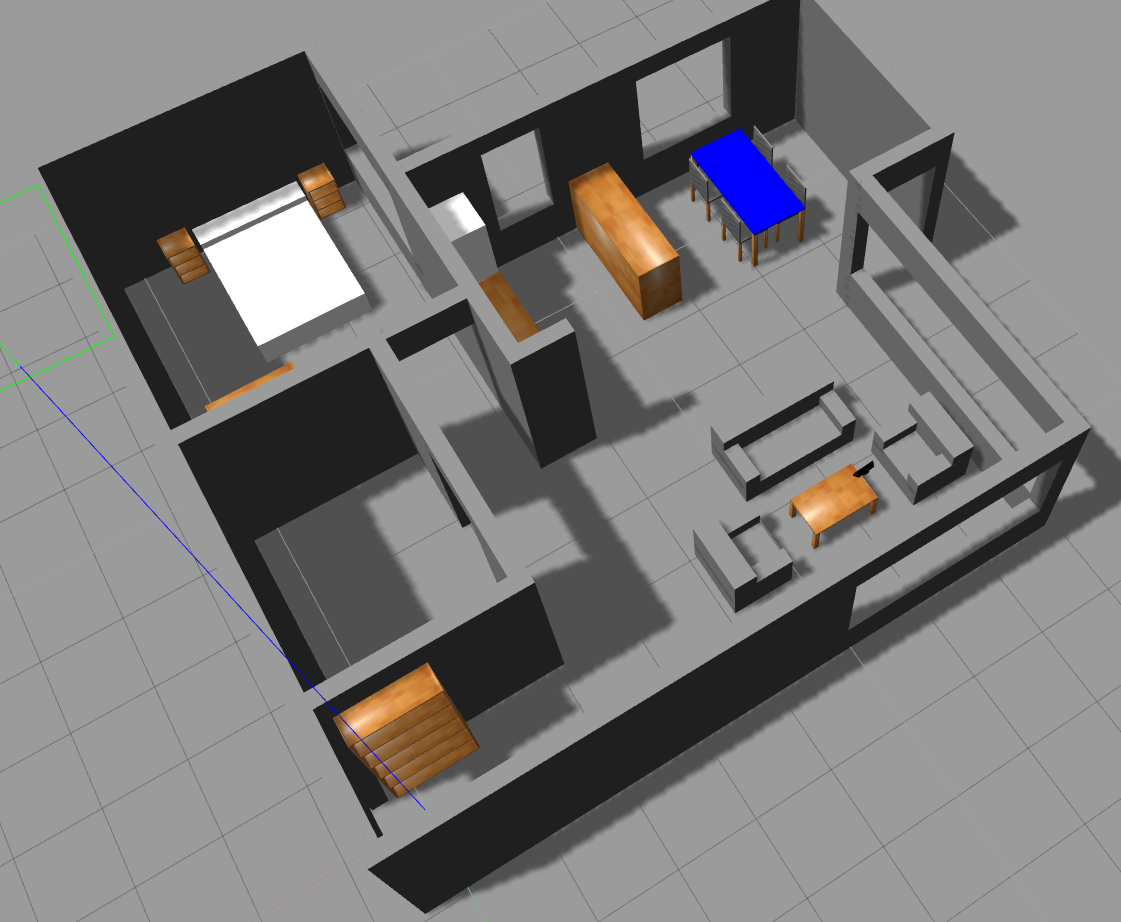
\includegraphics[width=0.6\textwidth]{figures/Vacuum/ModeloCasa_antiguo.png}
		\caption{Mundo GrannyAnnie.world en Gazebo}
		\label{fig.modelocasa_antiguo}
		\end{center}
\end{figure}

Primero había puertas que daban al exterior de la casa, entonces si pusiéramos a nuestra aspiradora a recorrer la casa se podría salir de la misma y no queremos que suceda esto. Segundo, se modificó el modelo de la casa debido a que había alguna pared que tenía mal la malla de colisiones, esto hacía que el robot pudiera atravesar algunas paredes. Se modificó la malla de colisiones en algunas zonas de la casa. Tercero, se modificaron las masas del inmobiliario incrementando su valor. Esto se debe a que la masa que tenían anteriormente no era suficiente y la aspiradora al colisionar con los muebles (mesas, sillones, etc) los desplazaba. El nuevo modelo de casa se llama ``house\_int2'' y lo podemos ver en la figura ~\ref{fig.casa}, donde aparecen los cambios marcados con un círculo rojo.\\

\begin{figure}[H]
  \begin{center}
    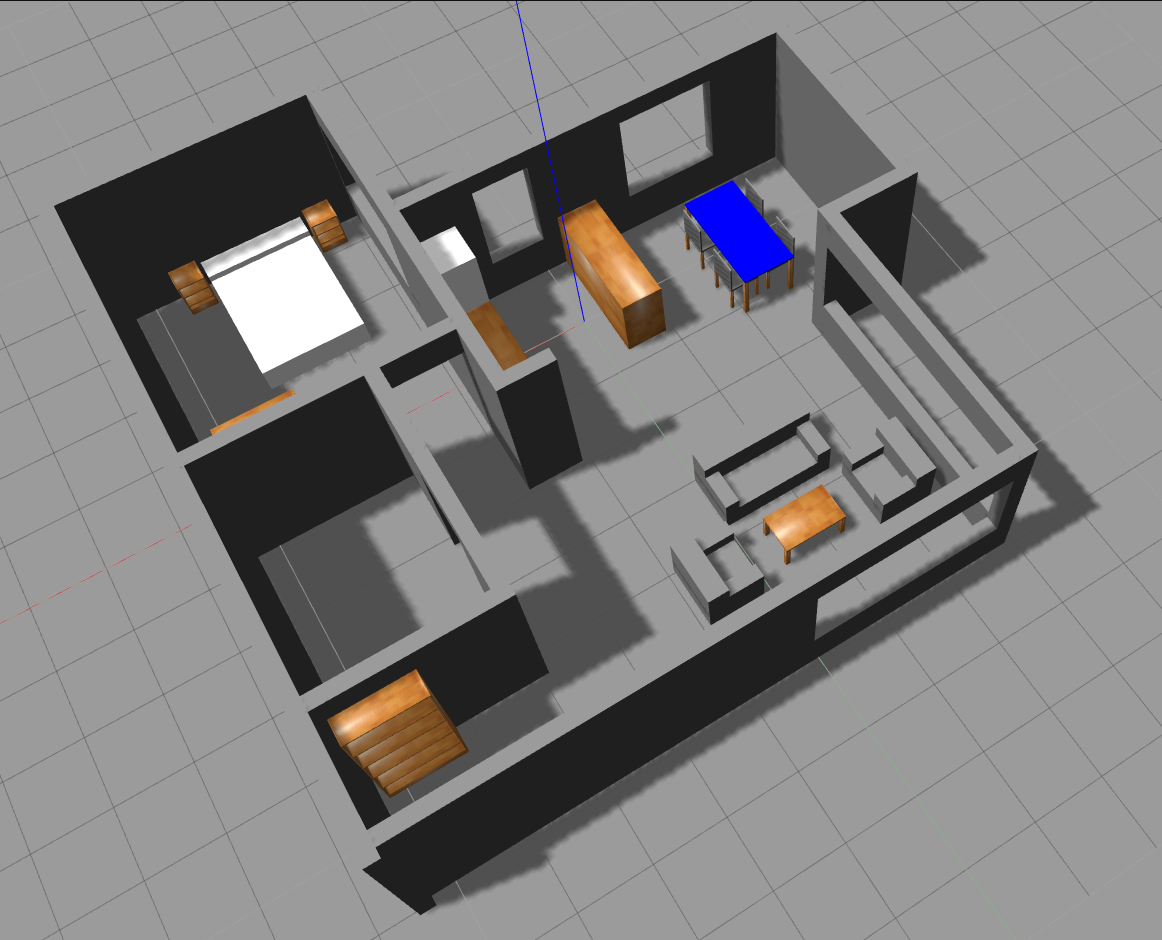
\includegraphics[width=0.6\textwidth]{figures/Vacuum/casa.png}
		\caption{Modelo house\_int2 en Gazebo}
		\label{fig.casa}
		\end{center}
\end{figure}

\subsection{Mundo de Gazebo}
Si queremos ver el comportamiento de la aspiradora dentro de la casa, antes debemos crear un mundo de Gazebo que esté formado por el modelo de la casa ``house\_int2'' y el modelo de aspiradora ``Roomba''. Por este motivo se ha creado un mundo llamado ``Vacuum.world''. En este mundo se incluyen luces. El archivo del mundo tiene el siguiente aspecto:

\vspace{20pt}
	\begin{lstlisting}[frame=single]
<?xml version="1.0" ?>
  <sdf version='1.4'>
    <world name=' Vacuum '>
    <include>
      <uri>model://roomba</uri>
        <pose>-1 1.5 0 0 0 0</pose>
    </include>
    <include>
      <uri>model://house_int2</uri>
        <pose>0 0 0 0 0 0</pose>
    </include>
    <include>
      <uri>model://ground_plane</uri>
   </include>

   <light name='sun' type='directional'>
       <cast_shadows>1</cast_shadows>
       <pose>0 0 10 0 -0 0</pose>
       <diffuse>0.8 0.8 0.8 1</diffuse>
       <specular>0.2 0.2 0.2 1</specular>
       <attenuation>
       <range>1000</range>
       <constant>0.9</constant>
       <linear>0.01</linear>
       <quadratic>0.001</quadratic>
       </attenuation>
       <direction>-0.5 0.1 -0.9</direction>
    </light>

    <scene>
        <ambient>0.4 0.4 0.4 1</ambient>
        <background>0.7 0.7 0.7 1</background>
        <shadows>1</shadows>
    </scene>

    <gui fullscreen='0'>
        <camera name='user_camera'>
            <pose>0.126197 6.13852 18.8314 0 1.08764 -2.14299</pose>
            <view_controller>orbit</view_controller>
        </camera>
    </gui>
    </world>
  </sdf>

	\end{lstlisting}

\section{Componente académico}
El componente académico resuelve varias funcionalidades auxiliares en la práctica: ofrece una interfaz gráfica al usuario que le ayuda a depurar su código; ofrece acceso a sensores y actuadores en forma de métodos simples (oculta el middleware de comunicaciones); incluye código auxiliar que no es el foco del algoritmo y que ayuda a programar la solución. El componente deja todo preparado para que el estudiante sólo tenga que retocar en MyAlgorithm.py.\\

Este componente ofrece al programador del algoritmo un \acrshort{api} de sensores y actuadores. A continuación, se puede ver el \acrshort{api} concreto de esta práctica:

\begin{itemize}
\item pose3d.getYaw(): Permite obtener la orientación del robot con respecto al mapa.
\item bumper.getBumperData().state: Devuelve un 1 si el robot colisiona y un 0 si no ha chocado.
\item laser.getLaserData(): Permite obtener los datos del sensor láser, que se compone de 180 pares de valores (0-180º, distancia en milímetros).
\item motors.sendV(): Para establecer la velocidad lineal.
\item motors.sendW(): Para establecer la velocidad de giro.

\end{itemize}


Este componente académico tiene un archivo de configuración (terminado con la extensión .cfg) que sirve para indicar los puertos que utilizan cada uno de los plugins que posee Roomba. Este archivo es necesario para que la aplicación pueda comunicarse con gazeboserver. Tiene el siguiente aspecto: 


\vspace{20pt}
	\begin{lstlisting}[frame=single]
VacuumCleaner.Motors.Proxy = Motors:default -h localhost -p 9003
VacuumCleaner.Pose3D.Proxy = Pose3D:default -h localhost -p 9003
VacuumCleaner.Laser.Proxy  = Laser:default -h localhost -p 9003
VacuumCleaner.Bumper.Proxy  = Bumper:default -h localhost -p 9003
VacuumCleaner.Motors.maxV = 5
VacuumCleaner.Motors.maxW = 20

	\end{lstlisting}
	
Tanto los motores, como la Pose3D, el láser y el bumper emplean el mismo puerto, el 9003. Gracias a cómo está configurado JdeRobot en su versión actual, se puede emplear el mismo puerto. Además, se puede observar que se establece la velocidad de tracción y rotación máxima que tendrán los motores de la aspiradora.\\

El componente emplea hilos de ejecución para realizar diferentes tareas al mismo tiempo, ya que se divide el comportamiento en tareas más sencillas. Esta práctica emplea varios procesos:

\begin{itemize}
\item Hilo de control: Es el encargado de actualizar los datos de los sensores y los actuadores a través de las interfaces \acrshort{ice}. El tiempo de refresco de este hilo es crucial, y tiene que ser muy corto, ya que este componente se encarga de establecer la velocidad y la dirección del robot en todo momento, así como de actualizar los datos de los sensores. Si este tiempo fuera muy grande, las decisiones que modifican la navegación del robot podrían ser incorrectas. EE hilo de control de actuadores y sensores se actualiza cada vez que se actualiza la \acrshort{gui}, es decir, cada 50 ms.

\item	Hilo de la interfaz gráfica de usuario (\acrshort{gui}): Este hilo es el encargado de actualizar la interfaz gráfica. También consta de los manejadores de eventos del \acrshort{gui}. El intervalo de actualización de la interfaz debe ser pequeño, ya que se tiene que mostrar la posición del robot en el mapa que se muestra en la interfaz en tiempo real. Este intervalo de tiempo es de 50 ms.

\end{itemize}


\subsection{Interfaz gráfica de la práctica}
La interfaz gráfica de usuario (\acrshort{gui}) de la práctica sirve para representar información importante de ayuda para resolver adecuadamente el algoritmo. La \acrshort{gui} se ha programado en Python con PyQt5.\\

En la \acrshort{gui}~\ref{fig.GUI2} de la práctica se muestra en la esquina superior izquierda el logo de JdeRobot. \\

\begin{figure}[H]
  \begin{center}
    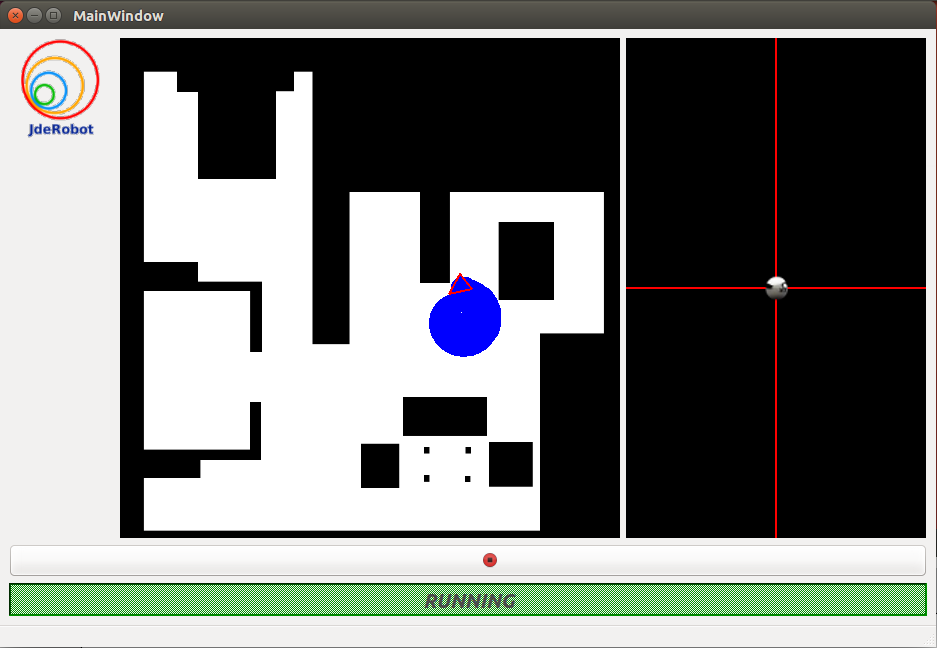
\includegraphics[width=0.7\textwidth]{figures/Vacuum/GUI2.png}
		\caption{Interfaz gráfica (\acrshort{gui}) de Vacuum después de un tiempo de ejecución}
		\label{fig.GUI2}
		\end{center}
\end{figure}

Contiene también una imagen del mapa de la casa por la que navega Roomba. Este mapa es una imagen binaria, donde aparecen con un color negro (valor 0) los obstáculos de la casa, mientras que el suelo, que es la zona por donde podrá navegar la aspiradora, tiene un color blanco (valor 255). Esta imagen es un simple visor de la situación de la aspiradora, ya que este mapa no se proporciona al alumno para la solución de la práctica. En el mapa también aparecerá pintada la posición de Roomba como un triángulo (donde solamente se pintan sus aristas) en color rojo. Esto permitirá saber dónde está situada nuestra aspiradora en el mapa, así como la orientación que tiene. También se pintarán en color azul las zonas de la casa por donde ha pasado la aspiradora. Esto ayudará a ver que hay por zonas por las que puede que haya pasado varias veces, mientras que por otras aún no habrá pasado.\\

Para pintar tanto el triángulo como las zonas por donde ha pasado el robot en el mapa hay que emplear un sistema de conversión del sistema de referencia del mundo (3D) al sistema de referencia del mapa (2D). Para pasar del sistema de referencia del mundo al del mapa se han empleado matrices de rotación y traslación, como sucedía en el capítulo ~\ref{cap.gpp}. En el caso de esta práctica los sistemas de referencia están situados de la siguiente forma:

\begin{figure}[H]
  \begin{center}
    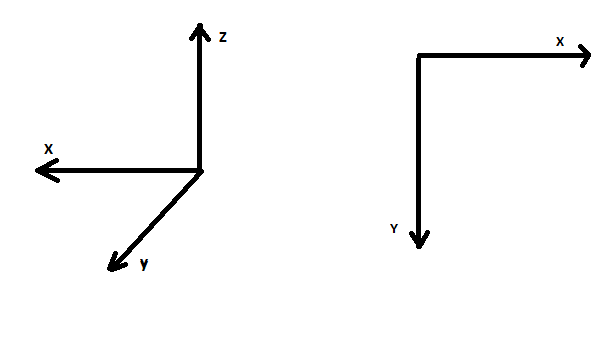
\includegraphics[width=0.6\textwidth]{figures/Vacuum/SistemaRef_world_image.png}
		\caption{Sistema de referencia del mundo (izquierda) y sistema de referencia de la imagen (derecha)}
		\label{fig.sistemaref_world}
		\end{center}
\end{figure}

Para saber dónde está situado nuestro robot en la imagen tenemos que pasar de una coordenada (x, y, z) en 3D a una coordenada (x’, y’) en 2D. En concreto, se aplica una rotación de pi grados (será el ángulo \(\alpha\) de la matriz) sobre el eje y. La traslación se realiza porque queremos tener el punto (0,0) de la imagen en la esquina superior izquierda, y para que se corresponda correctamente cada punto de la imagen con cada punto del mundo. En este caso la traslación que se ha aplicado es de 0.6 (será tx) en el eje x; y -1 (será ty) en el eje y. La matriz de rotación y traslación sobre el eje y es la siguiente:


\begin{equation}
\left[\begin{array}{cc}
x' \\ 
y' \\
z' \\
1
\end{array}\right] = \left[\begin{array}{cccc}
\cos(\alpha) & 0 & \sin(\alpha) & tx \\ 
0 & 1 & 0 & ty\\
-\sin(\alpha) & 0 & \cos(\alpha) & tz \\
0 & 0 & 0 & 1
\end{array}\right]* \left[\begin{array}{cc}
x \\ 
y \\
z \\
1
\end{array}\right]
\end{equation}
\\

De esta forma podemos pintar el triángulo, representación de la aspiradora, pasando la coordenada del mundo que nos devuelve el pose3d a coordenada en la imagen, la cual será el centro del triángulo que dibujaremos con una pequeña desviación. El triángulo es isósceles para distinguir cuál es la orientación del robot. La aspiradora estará orientada hacia el vértice que posee un ángulo menor que el resto.\\

Esta rotación también sirve para pintar en azul los puntos del mapa por donde ha pasado la aspiradora en cualquier momento. Se pintará un círculo en cada iteración dado que la aspiradora ocupa un determinado volumen. Los puntos por los que ha pasado la aspiradora se guardan en un array para saber por dónde ha pasado y pintarlos todos en cada iteración.\\

Por otra parte, en la esquina superior derecha de la \acrshort{gui}, tenemos un teleoperador para teleoperar el robot. Este teleoperador controla las velocidades lineal y angular del robot. La velocidad lineal del robot se puede controlar moviendo el joystick en sentido vertical. Cuanto más subamos el joystick más velocidad tendrá el robot hacia delante, y si lo bajamos del todo más velocidad lineal tendrá el robot hacia atrás. La velocidad angular del robot se controla moviendo el joystick en sentido horizontal, según lo movamos a izquierda o a la derecha, el robot girará en un sentido u otro.\\

En la aplicación gráfica hay además dos botones que son importantes. El botón superior, que aparece con un símbolo de stop, es el que emplearemos cuando teledirigimos a la aspiradora y queremos que pare en un punto y no siga navegando. El botón inferior, en el cual pone ``Run my algorithm'', es el botón con el que le ordenaremos al componente que comience a ejecutar la solución que se ha programado en el fichero MyAlgorithm.py. Este botón cambia de color al pulsarlo. Si queremos que este código pare en un determinado momento, pulsaremos el mismo botón haciendo que pare; y si queremos reanudar su comportamiento lo volveremos a pulsar.\\


\subsection{Gráfica de la derivada del porcentaje}
Para ayudar con la comprensión del desempeño del algoritmo de navegación se ha incluido en el \acrshort{gui} una gráfica de la derivada del porcentaje en función del tiempo. Con ella se puede comprobar cómo evoluciona el porcentaje de casa recorrido durante el tiempo, el ``rendimiento'' de la navegación. Esta gráfica es una ventana opcional dentro del \acrshort{gui} del componente académico. \\

En el caso de nuestra práctica, siguiendo esta definición de la derivada, podemos definir la derivada del porcentaje (eje vertical) respecto del tiempo (eje horizontal) como la diferencia del porcentaje cada unidad de diferencia del tiempo.\\

En este caso, en el eje horizontal se representa el tiempo, el cual se divide en 9 intervalos de tiempo. Cada intervalo de tiempo que se representa, en el eje horizontal, se corresponde con un intervalo de 100 segundos. Por lo tanto, en la práctica vamos a observar el comportamiento del porcentaje a lo largo de 900 segundos, es decir, 15 minutos.\\

En el eje vertical, se representa la diferencia de porcentaje en cada intervalo de tiempo. Es decir, por ejemplo, en el primer intervalo de tiempo se representará la diferencia de porcentaje recorrido entre el segundo 100 de la práctica y el segundo 0, en el segundo intervalo la diferencia entre el segundo 200 y el 100,etc.\\

Esta gráfica nos permitirá ver cómo evoluciona el porcentaje recorrido respecto al tiempo. Cuando la aspiradora realiza el algoritmo de navegación puede que en ciertas ocasiones pase varias veces por una misma zona o se quede un rato atascada en ciertas zonas. Al principio cuando ejecutamos la práctica es muy sencillo que nuestra aspiradora recorra un gran porcentaje de casa, pero más adelante será más complicado que pase por zonas por las que no había pasado aún. Esto implica que posiblemente la derivada del porcentaje en función del tiempo sea mayor al comienzo de la ejecución de la práctica que por el final. Cada vez que se ejecute la práctica esta gráfica variará.\\

En la Figura~\ref{fig.grafica_percentaje2} se puede observar un ejemplo de la gráfica de la derivada del porcentaje recorrido en función del tiempo.\\

\begin{figure}[H]
  \begin{center}
    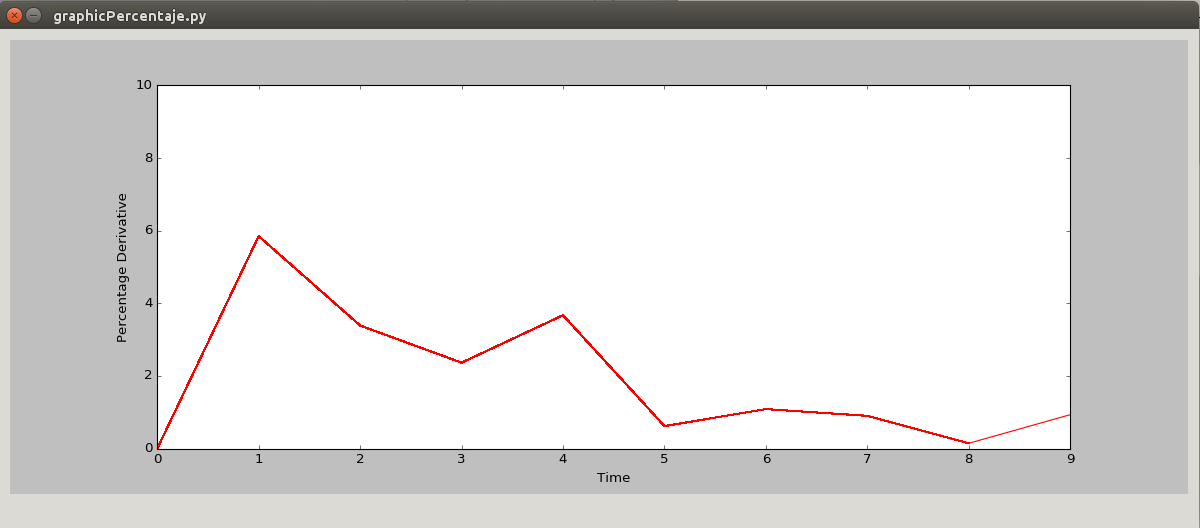
\includegraphics[width=0.9\textwidth]{figures/Vacuum/Grafica_percentaje2.png}
		\caption{Gráfica de la derivada del porcentaje en función del tiempo}
		\label{fig.grafica_percentaje2}
		\end{center}
\end{figure}

\section{Solución de referencia}
En este punto abordaremos una breve explicación sobre algoritmos que emplean aspiradoras robóticas disponibles en el mercado, una descripción de la técnica que emplea Roomba de iRobot, y la solución de referencia que se ha desarrollado para la práctica. 


\subsection{Algoritmos empleados por distintas aspiradoras robóticas}
En los últimos 15 años, han aparecido múltiples modelos de aspiradoras robóticas, las cuales son cada vez más innovadoras. Es importante tener en cuenta los algoritmos de navegación que llevan a cabo cada uno de los modelos, ya que en función de estos algoritmos la aspiradora limpiará en menor o mayor tiempo la casa. Además, es importante tener en cuenta en estos algoritmos los posibles obstáculos con los que se encontrará la aspiradora al recorrer la casa. A continuación, podemos ver diferentes algoritmos de navegación que existen hoy en día en función del modelo:

\begin{itemize}
\item Uno de los primeros modelos de aspiradora Trilobite de Electrolux navega empleando ultrasonidos. Esta aspiradora usa la siguiente estrategia de navegación: explora el perímetro del entorno (siguiendo un comportamiento de sigue la pared); después de que la aspiradora llegue al punto de partida donde comenzó a recorrer la pared, el robot estima el tamaño del entorno y comienza con una trayectoria aleatoria.
\begin{figure}[H]
  \begin{center}
    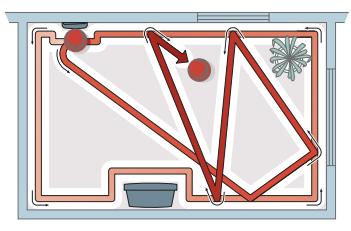
\includegraphics[width=0.6\textwidth]{figures/Vacuum/Trilobite.png}
		\caption{Patrón de navegación de la aspiradora Trilobite}
		\label{fig.Trilobite}
		\end{center}
\end{figure}
\item El sistema de navegación de la aspiradora robótica Xiaomi está guiado por un láser. Utiliza el algoritmo \acrfull{slam} para generar un mapa de la casa en la que se encuentra y calcula patrones inteligentes para moverse a través de la casa. Xiaomi afirma que su modelo de aspiradora no solamente sigue un mapa y trata de limpiar el 100\% de la superficie del suelo de la casa, sino que su aspiradora puede pensar y calcular el mejor patrón de limpieza para la casa.  Cuando arranca Xiaomi, hace un escaneo de la zona circundante y divide la habitación en secciones de aproximadamente 4 por 4 metros. A continuación, el robot realiza un barrido del perímetro alrededor de esta área seccionada, trazando los obstáculos que puedan interponerse en el camino de la trayectoria. Después, ``rellena'' esta sección haciendo barridos horizontales.
\begin{figure}[H]
  \begin{center}
    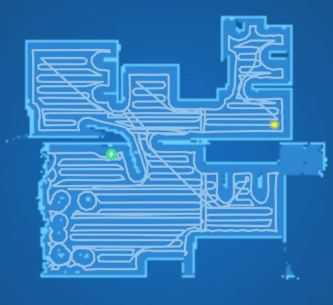
\includegraphics[width=0.4\textwidth]{figures/Vacuum/Xiaomi.png}
		\caption{Patrón de navegación de la aspiradora Xiaomi}
		\label{fig.Xiaomi}
		\end{center}
\end{figure}
\item También es importante destacar la gama de robot LG Hombot. Vamos a analizar en concreto el sistema de navegación del LG Hombot Turbo. Este aspirador es capaz de crear un mapa de la superficie, memorizando cada obstáculo, evitando el movimiento aleatorio y minimizando los choques. 
\item El más conocido de las aspiradoras robóticas es Roomba de iRobot. Roomba posee diferentes modelos, desde los más antiguos hasta los más innovadores. Existen grandes diferencias entre estos en cuanto a su patrón de limpieza. Los modelos de las series 500, 600, 700 y 800, calculan la ruta de limpieza óptima y determinan cuándo es necesario utilizar sus diversos modos de limpieza: giro en espiral, seguimiento de paredes, cruce de habitación. En cambio, los modelos de la serie 900 de Roomba, tienen navegación iAdapt 2.0, se adaptan al entorno y disponen de localización visual para limpiar. A través de la localización visual, crea un mapa con referencias para recorrer toda la casa y saber por dónde ha pasado y dónde tiene que ir. Limpia de forma eficiente en áreas abiertas moviéndose en líneas paralelas mientras que, gracias a los sensores, adapta su trayectoria cuando se necesita limpiando de forma eficiente.
\end{itemize}

Estos modelos que acabamos de mencionar son solamente unos pocos dentro de una amplia variedad de modelos de aspiradoras robóticas que existen hoy en día. Es importante destacar que todos los modelos de aspiradora usan diferentes modos de limpieza (espiral, zig-zag, aleatorio, recorrer bordes, etc) en función de la zona de la casa donde se encuentren o en función de qué es lo que más le interesa a su dueño. Existen modelos de aspiradoras que emplean patrones aleatorios para poder limpiar la casa; y, por otro lado, hay otros modelos que inicialmente se construyen un mapa de la casa para recorrer la superficie de una forma más óptima.

\subsection{Algoritmo empleado por Roomba serie 500, 600, 700, 800}
Para resolver el algoritmo sin autolocalización que se plantea en la práctica nos hemos basado en el algoritmo de navegación que siguen los modelos de las series 500, 600, 700 y 800 de Roomba, que no emplean un mapa de la casa.\\

Mientras Roomba está limpiando evita caerse por las escaleras o por un terreno empinado. Esto lo hace gracias a cuatro sensores infrarrojos en la parte inferior delantera. Estos sensores envían constantemente señales de infrarrojos, y si estas señales se pierden es porque el robot ha llegado a una zona de elevada pendiente por donde podría caerse.\\

Cuando Roomba choca con un objeto el \textit{bumper} se retrae, activando sensores de objetos mecánicos que le avisan a Roomba de que ha chocado. Cuando se produce este hecho la aspiradora gira y avanza hasta que encuentra una ruta despejada.\\

Esta aspiradora tiene otro sensor de infrarrojos (llamado \textit{Wall sensor}) situado en la parte delantera del robot. Este sensor permite que Roomba navegue muy de cerca de las paredes, los objetos, etc. \\

Cuando presionamos el botón ``Clean'', lo primero que hace Roomba es calcular el tamaño de la habitación según la información que recibe a través de sus sensores. Este robot envía una señal infrarroja y comprueba el tiempo que tarda en volver la señal. De esta manera calcula el tiempo que tendrá que pasar limpiando. Esto le permite optimizar la cobertura por habitación. El tiempo de funcionamiento que calcula depende del tamaño de la habitación y de la carga de la batería. \\

Roomba ejecuta su algoritmo 67 veces por segundo, obteniendo constantemente la información sobre su entorno y recomponiendo su trayectoria.\\

Roomba comienza a limpiar siguiendo un patrón de espiral. Esta espiral se va haciendo cada vez más grande, saliendo la espiral hacia fuera sobre un área más grande y más grande hasta que golpee un objeto. Cuando Roomba encuentre un objeto, seguirá a lo largo de este objeto recorriendo el perímetro de la habitación durante un periodo de tiempo determinado. Cuando pase este periodo de tiempo, comenzará el modo cruce de la habitación, tratando de averiguar la máxima distancia que puede navegar sin chocar con un objeto. Sin embargo, si lleva un periodo de tiempo grande navegando sin chocarse con ningún obstáculo va a comenzar otra vez a realizar la espiral, porque supone que está en un amplio espacio abierto.\\

Estos patrones que eligieron los creadores de Roomba se basan en los algoritmos basados en los comportamientos de los animales cuando van buscando áreas de comida. Es bastante eficaz y robusto en situaciones del mundo real. A continuación, podemos observar en la imagen ~\ref{fig.Algoritmo_roomba} el patrón de comportamiento que sigue Roomba.\\

\begin{figure}[H]
  \begin{center}
    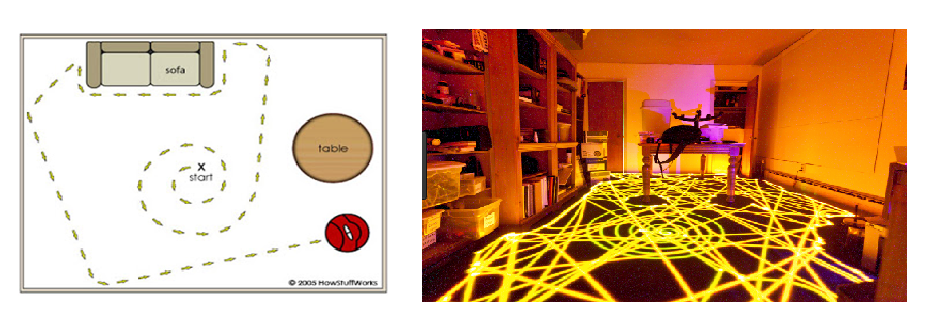
\includegraphics[width=1\textwidth]{figures/Vacuum/Algoritmo_roomba.png}
		\caption{Algoritmo de navegación de Roomba}
		\label{fig.Algoritmo_roomba}
		\end{center}
\end{figure}

\subsection{Solución desarrollada}
La solución se desarrolla en el fichero ``MyAlgorithm.py''. En el método ``execute'', el cual se ejecuta periódicamente. De esta forma, el pilotaje se llevará a cabo como un control reactivo, es decir, la aspiradora podrá comprobar los datos de sus sensores en cada instante y basándose en estos datos optar por realizar una acción u otra. Podemos ver que no se realiza ningún tipo de planificación, sino que se lleva a cabo el pilotaje directamente, de modo reactivo.\\

El primer paso que lleva a cabo la solución desarrollada es realizar una navegación siguiendo un patrón en espiral (al igual que lo hacía la Roomba real). Si queremos realizar un patrón en espiral debemos elegir qué tipo de espiral queremos, ya que existen numerosos tipos. Algunos de los tipos son: espiral de Arquímedes, espiral logarítmica, espiral hiperbólica, espiral de Fermat, espiral de Durero, etc. En el caso de esta práctica se ha optado por realizar la espiral de Arquímedes, que es uniforme. Esta espiral se define como el lugar geométrico de un punto moviéndose a velocidad constante sobre una recta que gira sobre un punto de origen fijo a velocidad angular constante. En la figura ~\ref{fig.Espiral_Arquimedes} se puede ver el patrón que sigue la espiral de Arquímedes.\\

\begin{figure}[H]
  \begin{center}
    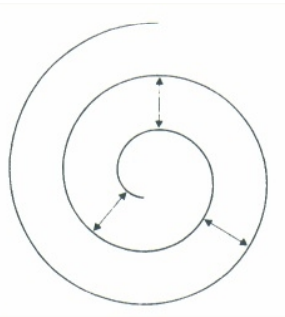
\includegraphics[width=0.3\textwidth]{figures/Vacuum/Espiral_Arquimedes.png}
		\caption{Espiral de Arquímedes}
		\label{fig.Espiral_Arquimedes}
		\end{center}
\end{figure}

Para que la aspiradora pueda realizar un patrón de este tipo, debe tener una velocidad angular constante y una velocidad lineal incremental. Es decir, la velocidad lineal irá aumentando en cada iteración un determinado valor. Se ha optado por tomar como velocidad lineal la multiplicación de dos valores (los cuales inicialmente son valores muy pequeños). Un valor de radio inicial será multiplicado por una variable, la cual irá aumentando en cada iteración. El valor del radio inicial es de 0.1, mientras que la variable inicialmente posee un valor de 0.01. Esta variable será incrementada un 0.012 en cada iteración. De esta forma obtenemos un patrón en espiral similar a la espiral de Arquímedes.\\

Esta espiral se va haciendo cada vez más grande, saliendo la espiral hacia fuera sobre un área más grande. Roomba seguirá este patrón en espiral hasta que choque con un obstáculo. En la figura ~\ref{fig.Espiral_Roomba} podemos ver el patrón en espiral que ha realizado la aspiradora.\\

\begin{figure}[H]
  \begin{center}
    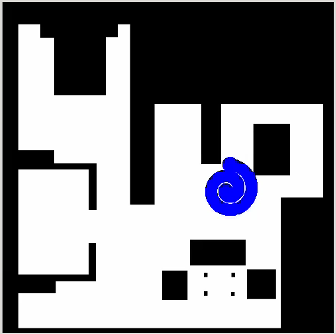
\includegraphics[width=0.5\textwidth]{figures/Vacuum/Espiral_Roomba.png}
		\caption{Espiral que realiza Roomba en la práctica}
		\label{fig.Espiral_Roomba}
		\end{center}
\end{figure}

Cuando Roomba choca con un obstáculo, sigue a lo largo del contorno de este obstáculo recorriendo el perímetro de la casa durante un determinado periodo de tiempo, 300 segundos. Se ha optado por esta duración porque en las pruebas que se han realizado es el que mejores resultados presentaba.\\

Para seguir el perímetro se han empleado los datos que recoge el sensor láser que posee Roomba. Para obtener los datos del sensor láser que emplea la función laser.getLaserData(). \\

En este subestado lo primero que hace Roomba es separarse un poco de la pared para no rozar todo el rato con ella. Después gira un poco hasta que encuentra que tiene la pared a su derecha. Para saber si tiene la pared a la derecha emplea el valor de distancia del ángulo 0 (rayo que está a la derecha de Roomba) y el ángulo 45 del array.\\

Tras saber que ya tenemos la pared a la derecha de la aspiradora, podemos recorrer el perímetro. Para ello hay que comprobar continuamente el láser frontal (situado en el ángulo 90). Si la aspiradora está en una esquina, la distancia que obtiene ese láser será muy pequeña. Si se da el caso de que se encuentra en una esquina, Roomba girará a la izquierda 90 grados. \\

Otro dato que comprobará es si el láser del ángulo 135 (más a la izquierda) tiene una distancia muy pequeña y además ha detectado un choque. Esto indica que la aspiradora se ha quedado enganchada en algún hueco. Si se da este caso la aspiradora retrocede un poco y gira hacia la izquierda 90 grados.\\

Si la aspiradora no se encuentra en una esquina y no se ha quedado atascada en algún hueco, entonces recorrerá el perímetro siguiendo la pared. Para ello, se comprueba el láser derecho (ángulo 0) y el láser del ángulo 45. Este algoritmo se realiza de forma reactiva comprobando continuamente los datos y tomando decisiones en base a ellos. Si la distancia a la pared es demasiado pequeña es que estamos muy pegados a la pared. En este caso la aspiradora gira un poco a la izquierda para no chocarse con la pared. Si el valor de distancia es muy grande, entonces gira un poco a la derecha para no desviarse de la pared. Si la distancia a la pared no es ni muy pequeña, ni muy grande, es que podemos seguir adecuadamente la pared tomando una velocidad lineal constante y una velocidad angular nula.\\

Teniendo en cuenta todas estas situaciones que se pueden dar al recorrer la pared, la aspiradora recorre el perímetro correctamente. En la siguiente figura ~\ref{fig.Perimetro_Roomba} se puede ver cómo después de realizar el patrón en espiral, Roomba ha realizado el perímetro durante un intervalo de tiempo.\\

\begin{figure}[H]
  \begin{center}
    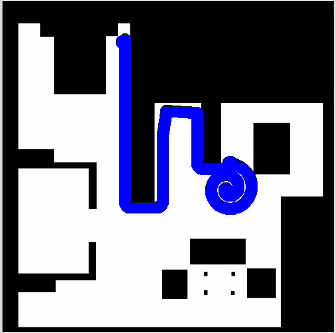
\includegraphics[width=0.5\textwidth]{figures/Vacuum/Perimetro_Roomba.png}
		\caption{Perímetro que recorre Roomba en la práctica}
		\label{fig.Perimetro_Roomba}
		\end{center}
\end{figure}

El siguiente subestado que se lleva a cabo es un algoritmo aleatorio, que realiza un cruce de habitación (similar a la Roomba real). Lo que hace en este caso Roomba es comprobar continuamente si la aspiradora ha chocado o no , en cada iteración. Si ha chocado entonces retrocede un poco para apartarse de la pared, y calcula un ángulo aleatorio y el signo aleatoriamente. Este ángulo es el que girará Roomba para tomar una nueva orientación El signo que calculamos aleatoriamente es para que nuestra aspiradora gire algunas veces hacia la izquierda y otras veces a la derecha, dotando al algoritmo de mayor aleatoriedad. Para elegir el signo se emplea una función que proporciona Python para calcular aleatoriamente números enteros. En este caso se define un número entre 0 y 1. Si el signo sale 0, entonces Roomba gira a la derecha; si por el contrario es 1, gira a la izquierda.\\

Tras calcular el ángulo y el signo aleatoriamente, Roomba gira hasta haber girado el ángulo que se le ha indicado. Cuando ha realizado el giro, la aspiradora toma como velocidad de giro 0 y toma una velocidad lineal constante. De esta forma Roomba irá recta hacia la orientación que se haya quedado después del giro. Roomba seguirá la recta hasta que vuelva a chocar. Cuando choque volverá a realizar el algoritmo aleatorio hasta finalizar el tiempo de la práctica.\\


\section{Evaluador automático}
Se ha creado un evaluador automático que en función de diferentes parámetros califica el algoritmo que ha programado el alumno como solución. El evaluador automático muestra en una interfaz gráfica diferentes parámetros, así como la nota final que obtiene el alumno. Este evaluador automático se ha creado utilizando PyQt5 al igual que el componente académico. Para programarlo se han creado clases diferentes para cada parámetro que queramos mostrar en la interfaz. Estas clases serán instanciadas en una clase principal (llamada MainWindow), que contiene la ventana principal del evaluador.\\

En la esquina superior izquierda de la figura ~\ref{fig.Referee_Vacuum2}, tiene un visor que muestra una barra de progreso. En esta barra se pinta en rojo el porcentaje de superficie recorrida por la aspiradora en cada momento. Encima de esta barra se mostrará esa misma información de modo numérico. El porcentaje de superficie recorrida se calcula teniendo en cuenta que el 100\% es el suelo donde no hay obstáculos situados. Es decir, todos los píxeles en blanco que aparecen en el mapa que muestra la interfaz.\\

En la esquina inferior izquierda se muestra la imagen del mapa de la casa. Los píxeles blancos (valor 255) representan la zona libre de obstáculos por donde puede navegar la aspiradora (el suelo). Los píxeles en negro (valor 0) representan a los obstáculos que hay en la casa. En esta imagen también se pinta en azul las zonas por donde ha pasado la aspiradora en cualquier momento. Para ello se guardan las posiciones por las que pasa en un array, y se pinta en cada iteración.\\

En la esquina superior derecha, tenemos un reloj digital, donde se muestran los segundos restantes hasta el final de la prueba. Los segundos van disminuyendo, es decir, se muestra una cuenta atrás de segundos. Este visor comienza mostrando 900 segundos (que son 15 minutos) y cada vez que ha pasado un segundo lo va descontando de este valor. Se ha considerado un intervalo de tiempo adecuado para evaluar la práctica, ya que si pusiéramos un intervalo mayor de tiempo sería un tiempo excesivo para evaluar la práctica. Si ponemos un intervalo de tiempo menor a 15 minutos no se podría evaluar la práctica con claridad, ya que en los primeros minutos de la práctica es muy sencillo recorrer bastante porcentaje de suelo comparando con los minutos posteriores.\\

Debajo de este visor del tiempo digital se muestra un visor de un reloj analógico. En este reloj analógico sí que avanza el tiempo.\\


Por último, hay que mencionar que cuando terminen los 900 segundos, a la derecha del reloj digital aparecerá un mensaje con la nota que ha obtenido el alumno. Esta nota se calculará en función del porcentaje recorrido por la aspiradora al pasar 900 segundos. Se ha establecido un porcentaje máximo para estos 15 minutos, ya que no es posible recorrer toda la casa en este tiempo. Si la aspiradora recorre un 30\% o más, el alumno obtendrá una nota de 10 puntos. Si por el contrario, la aspiradora recorre menos porcentaje, entonces se calcula la nota haciendo una regla de tres sabiendo que una nota de 10 es un 30\%.\\

En las Figura~\ref{fig.Referee_Vacuum2}, podremos ver el evaluador automático durante el pilotaje.

\begin{figure}[H]
  \begin{center}
    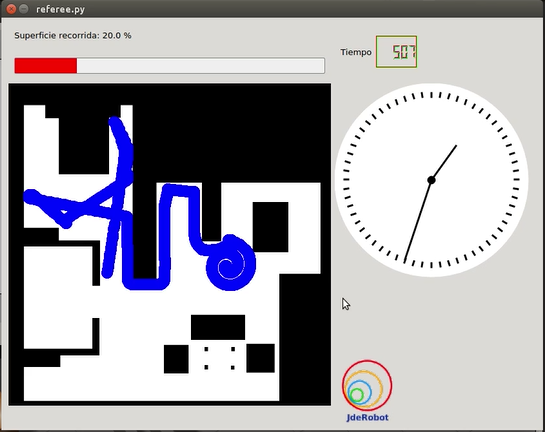
\includegraphics[width=0.6\textwidth]{figures/Vacuum/Referee_Vacuum2.png}
		\caption{Evaluador automático durante la ejecución de la práctica}
		\label{fig.Referee_Vacuum2}
		\end{center}
\end{figure}


\section{Experimentación}

\subsection{Ejecución típica}
La práctica se ejecuta abriendo cuatro terminales y escribiendo lo siguiente en cada uno de ellos: 
\begin{enumerate}[1.]
    \item Lanzar Gazebo: gazebo Vacuum.world
\end{enumerate}
\begin{enumerate}[1b.]
\item Si el ordenador que se emplea no tiene muchos recursos se puede arrancar el simulador sin interfaz gráfico: Lanzar Gazebo: gzserver Vacuum.world
\end{enumerate}
\begin{enumerate}[2.]
    \item Ejecutar el componente académico: python2 vacuumCleaner.py -- --Ice.Config = vacuumCleaner.cfg
\end{enumerate}
\begin{enumerate}[3.]
  	\item Ejecutar el evaluador automático: python2 referee.py -- --Ice.Config=vacuumCleaner.cfg
 \end{enumerate}

En la figura ~\ref{fig.Referee_Roomba} se puede observar el resultado del evaluador automático al finalizar la prueba tras evaluar la solución de referencia. Se puede observar que se consigue recorrer el 28\% de  la superficie, obteniendo una nota de 9.33. Además, al emplear en el último subestado de la solucion un algoritmo aleatorio podemos ver que la aspiradora no recorre únicamente una habitación, sino que navega por diferentes habitaciones.

\begin{figure}[H]
  \begin{center}
    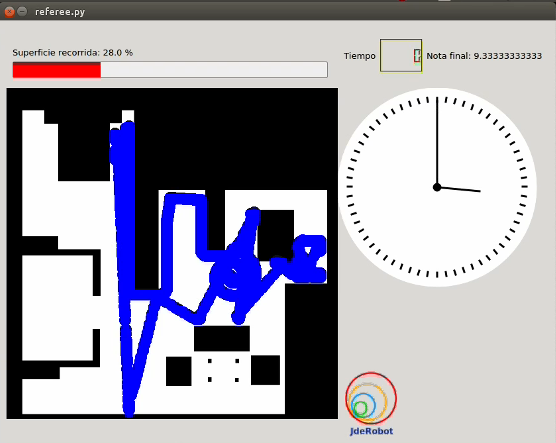
\includegraphics[width=0.7\textwidth]{figures/Vacuum/Referee_Roomba.png}
		\caption{Evaluador automático con la nota final}
		\label{fig.Referee_Roomba}
		\end{center}
\end{figure}

\subsection{Ajuste del tiempo de navegación perimetral}
Un punto importante de la práctica es decidir cuál es el periodo de tiempo que la aspiradora se mantendrá recorriendo el perímetro. En la práctica se ha optado por recorrer el perímetro durante 300 segundos. Para elegir un periodo de tiempo se han hecho pruebas con diferentes valores. Se han realizado tres pruebas por cada periodo de tiempo para sacar una media del porcentaje recorrido y elegir el periodo con mayor porcentaje, aunque al ser aleatorio si hiciéramos la prueba mil veces puede que saliera otro resultado, pero hemos elegido este periodo de 300 segundos en base a estas pruebas. Los periodos de tiempo en los que se han realizado pruebas para el perímetro son 200, 300, 400, 500 y 600 segundos. A continuación, se puede ver en la tabla ~\ref{resultados_roomba} los resultados obtenidos para cada periodo.\\


\begin{table}[]
\centering
\caption{Resultados}
\label{resultados_roomba}
\begin{tabular}{c|c|c|c|c|c|c|c|c|}
\cline{2-9}
                          & \multicolumn{2}{c|}{1º Prueba} & \multicolumn{2}{c|}{2º Prueba} & \multicolumn{2}{c|}{3º Prueba} & \multicolumn{2}{c|}{Media} \\ \cline{2-9} 
                          & Nota        & Porcentaje       & Nota        & Porcentaje       & Nota        & Porcentaje       & Nota      & Porcentaje     \\ \hline
\multicolumn{1}{|c|}{200} & 6.66        & 20 \%            & 10          & 33 \%            & 6           & 18 \%            & 7.55      & 23.66 \%       \\ \hline
\multicolumn{1}{|c|}{300} & 9.33        & 28 \%            & 8           & 24 \%            & 9           & 27 \%            & 8.77      & 26.33 \%       \\ \hline
\multicolumn{1}{|c|}{400} & 9.33        & 28 \%            & 8           & 14 \%            & 8.66        & 26 \%            & 8.66      & 26 \%          \\ \hline
\multicolumn{1}{|c|}{500} & 6.66        & 20 \%            & 8.33        & 25 \%            & 6           & 18 \%            & 7         & 21.66 \%       \\ \hline
\multicolumn{1}{|c|}{600} & 7.33        & 22 \%            & 7           & 21 \%            & 7.33        & 22 \%            & 7.22      & 21.66 \%       \\ \hline
\end{tabular}
\end{table}

En el caso del periodo de 200 segundos se puede ver que el 33\% es un gran resultado, que nos da como nota de calificación 10. Sin embargo, el resto de resultados obtenidos no son muy buenos, lo que hace que baje notablemente la nota. En la Figura~\ref{fig.Referee200} se puede ver la imagen del mapa con la superficie recorrida en azul para las tres pruebas mencionadas. En el caso de la segunda imagen se puede ver que hay más superficie recorrida.


\begin{figure}[H]
  \begin{center}
    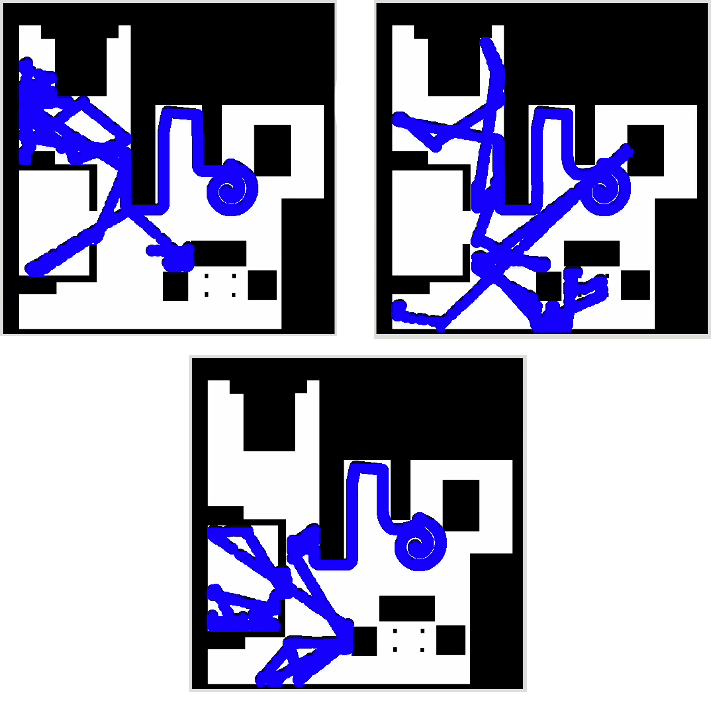
\includegraphics[width=0.7\textwidth]{figures/Vacuum/Referee200.png}
		\caption{Superficie recorrida de las pruebas de 200 segundos de perímetro}
		\label{fig.Referee200}
		\end{center}
\end{figure}

En la prueba del periodo de 300 segundos, vemos que tanto la nota como el porcentaje, es mayor en este caso que en el periodo de 200 segundos. En este caso no hemos obtenido en ninguna prueba una nota de 10 como en el periodo de 200 segundos, pero la media es mejor. En la Figura~\ref{fig.Referee300} vemos el mapa con la superficie recorrida para las tres pruebas realizadas.

\begin{figure}[H]
  \begin{center}
    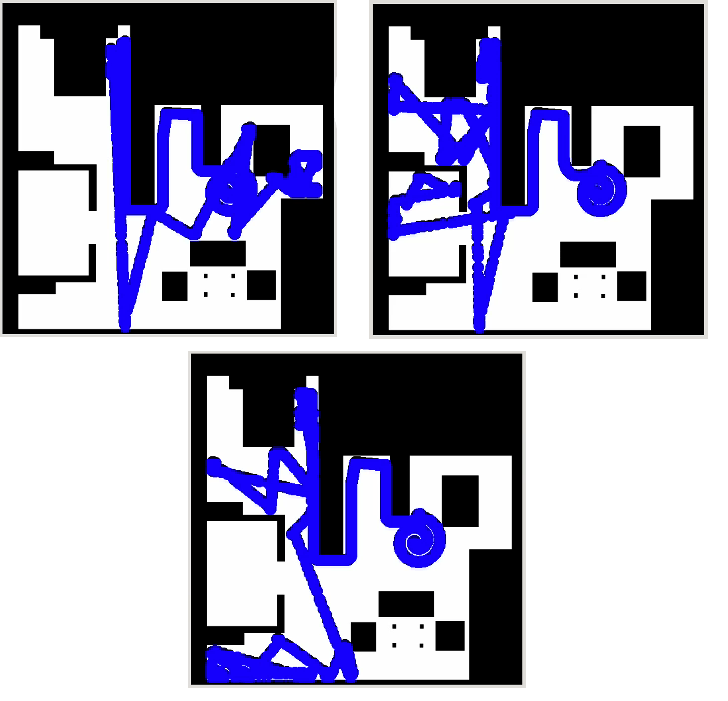
\includegraphics[width=0.7\textwidth]{figures/Vacuum/Referee300.png}
		\caption{Superficie recorrida de las pruebas de 300 segundos de perímetro}
		\label{fig.Referee300}
		\end{center}
\end{figure}

Cuando se han realizado pruebas con un periodo de 400 segundos para recorrer el perímetro, se han logrado resultados muy similares al periodo de 300 segundos, por lo que un periodo de 400 segundos también podría haberse empleado en la práctica, ya que da buenos resultados. En la Figura~\ref{fig.Referee400} se muestra el mapa con la superficie recorrida para cada una de las pruebas.

\begin{figure}[H]
  \begin{center}
    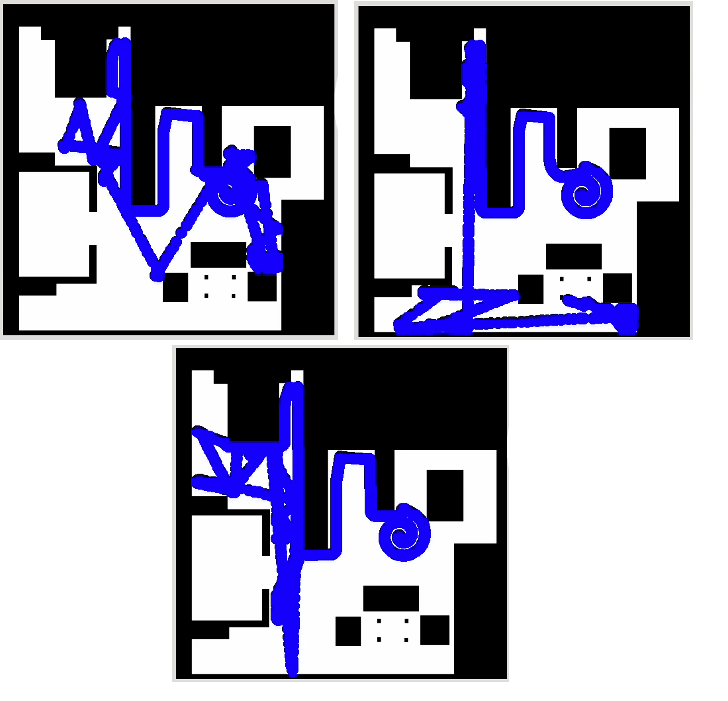
\includegraphics[width=0.7\textwidth]{figures/Vacuum/Referee400.png}
		\caption{Superficie recorrida de las pruebas de 400 segundos de perímetro}
		\label{fig.Referee400}
		\end{center}
\end{figure}

En el caso de emplear un periodo de 500 segundos, los resultados que se obtienen no son tan buenos como en los casos anteriores, por lo que se descartó usar este intervalo de tiempo. En la Figura~\ref{fig.Referee500} se ve el mapa con la superficie recorrida en cada caso.\\

\begin{figure}[H]
  \begin{center}
    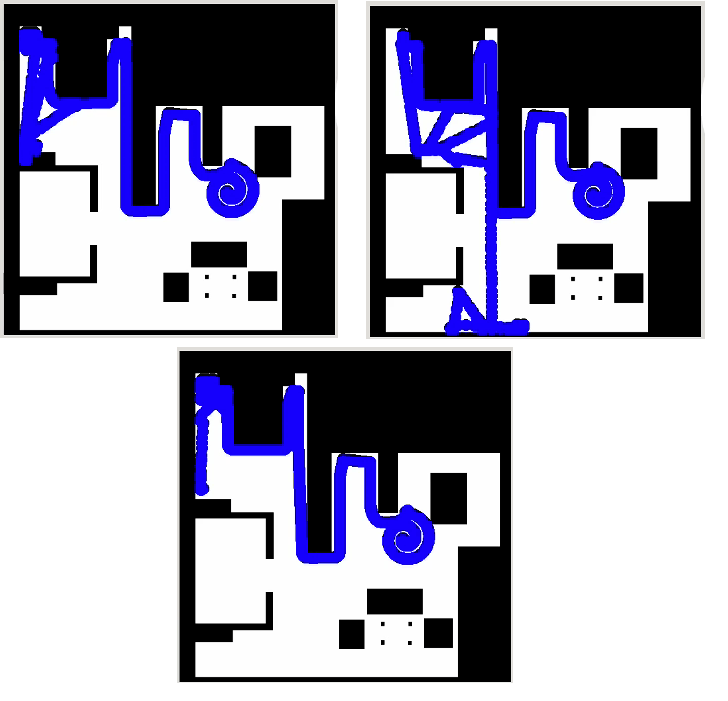
\includegraphics[width=0.7\textwidth]{figures/Vacuum/Referee500.png}
		\caption{Superficie recorrida de las pruebas de 500 segundos de perímetro}
		\label{fig.Referee500}
		\end{center}
\end{figure}

Por último, empleando un intervalo de tiempo de 600 segundos los resultados que se consiguen son similares a los obtenidos con un intervalo de 500 segundos. Podemos ver en la Figura~\ref{fig.Referee600} el mapa con la superficie recorrida por la aspiradora para las pruebas de 600 segundos. \\

\begin{figure}[H]
  \begin{center}
    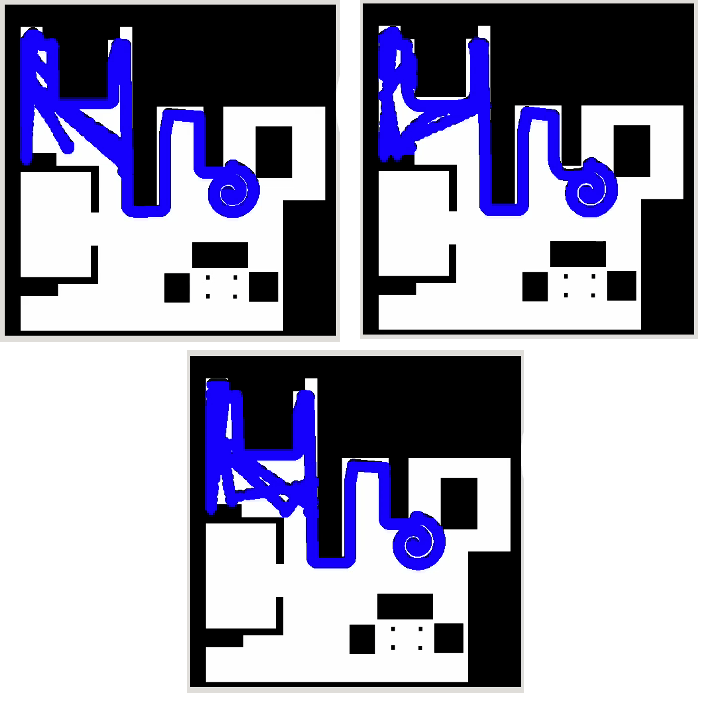
\includegraphics[width=0.7\textwidth]{figures/Vacuum/Referee600.png}
		\caption{Superficie recorrida de las pruebas de 600 segundos de perímetro}
		\label{fig.Referee600}
		\end{center}
\end{figure}

\subsection{Experimentos de 45 minutos}
Es importante mencionar que, si tuviéramos una casa sin obstáculos, sin paredes y sin ningún hueco donde se pudiera quedar atascada la aspiradora, entonces el porcentaje que podría recorrer la aspiradora sería mucho mayor. Esto se debe a que estos obstáculos hacen que la aspiradora se quede mucho tiempo en algunas zonas y no recorra otras. Es posible que la aspiradora navegue por una zona varias veces, y, sin embargo, no recorra otras zonas en estos 15 minutos.\\

Para comprobar la diferencia de porcentaje recorrido, se han hecho tres pruebas de 45 minutos, con el intervalo de perímetro de 300 segundos, por lo que la aspiradora realizará un algoritmo aleatorio durante mucho tiempo. \\

En las pruebas que se han realizado se han obtenido unos resultados de porcentaje del 49\%, 42\%, y 45\%. Estos porcentajes dan una media de 45.33\%. Por lo tanto, se puede ver que la media está cercana a la mitad de porcentaje de la casa. En la Figura~\ref{fig.Referee_45MIN} se puede ver el mapa con la superficie recorrida en las tres pruebas. En estas imágenes se puede observar que en algunas ocasiones hay algunas habitaciones donde la superficie ha sido recorrida casi en su totalidad.\\

\begin{figure}[H]
  \begin{center}
    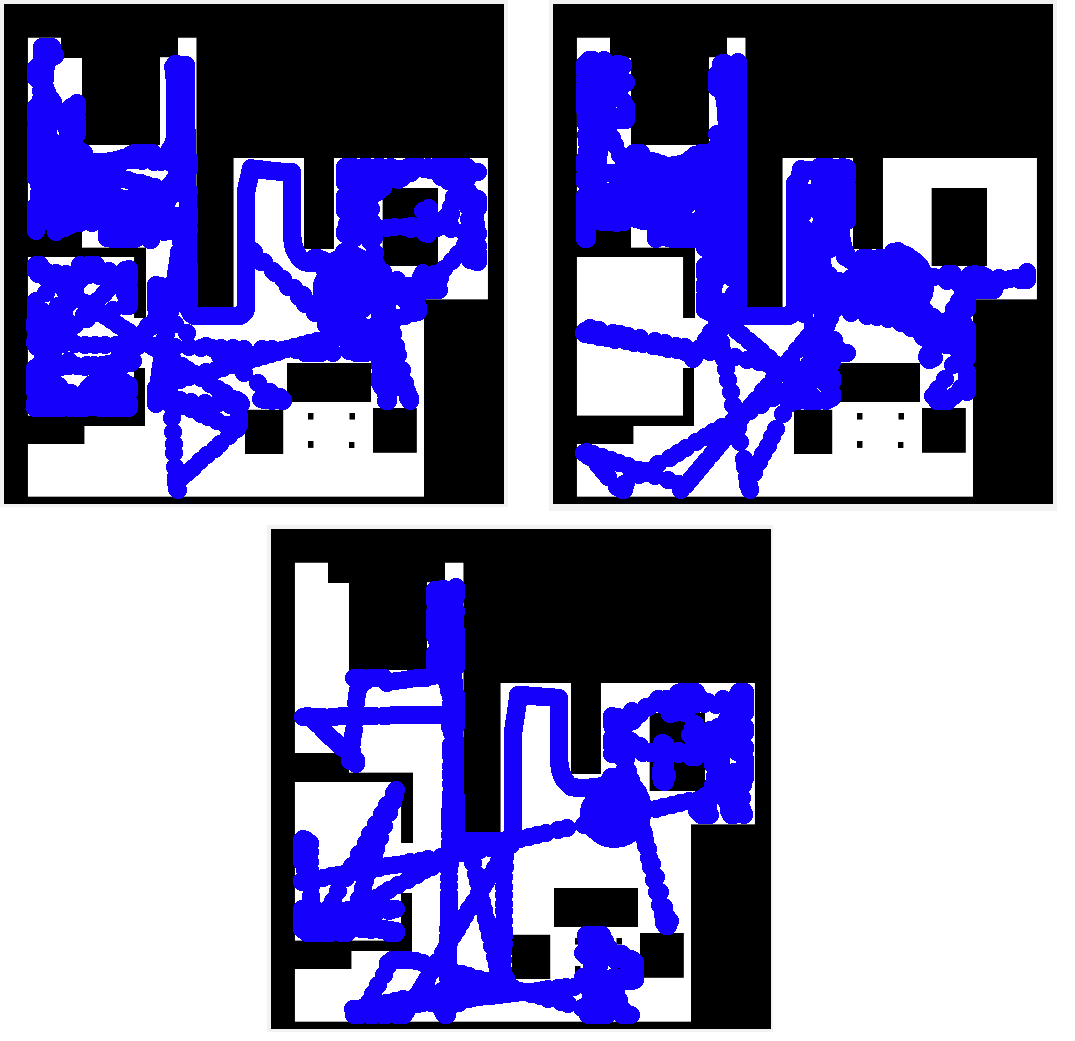
\includegraphics[width=0.7\textwidth]{figures/Vacuum/Referee_45MIN.png}
		\caption{Superficie recorrida de las pruebas de 45 minutos}
		\label{fig.Referee_45MIN}
		\end{center}
\end{figure}

\subsection{Ley de los rendimientos decrecientes}

Se ha estudiado el porcentaje recorrido en función de diferentes duraciones de tiempo. Viendo los porcentajes obtenidos en la prueba de 45 minutos se podría decir que si la aspiradora navegara durante hora y media podría llegar al 90\% o 100\% dependiendo de la ocasión. Pero no es así, la aspiradora tardaría más tiempo, ya quecada vez es más complicado alcanzar nuevos puntos en la casa por donde no haya pasado. Se han realizado varias pruebas de hora y media para comprobar el porcentaje recorrido. Hemos comprobado que existe una ley de rendimiento decreciente, lo que supone que a mayor tiempo de ejecución del algoritmo de solución menor será el rendimiento en cuanto a porcentaje recorrido. Este aspecto lo podemos ver en la tabla ~\ref{resultados_periodos}, donde comparamos las pruebas de 15, 45 y 90 minutos. En la Figura~\ref{fig.Referee_hora} se puede ver la superficie recorrida en las tres pruebas de 90 minutos.

\begin{table}[]
\centering
\caption{Resultados}
\label{resultados_periodos}
\begin{tabular}{c|c|c|c|c|c|c|c|c|}
\cline{2-4}
                          & \multicolumn{1}{c|}{1º Prueba} & \multicolumn{1}{c|}{2º Prueba} & \multicolumn{1}{c|}{3º Prueba} \\ \cline{2-4} 
                         & Porcentaje       & Porcentaje       & Porcentaje     \\ \hline
\multicolumn{1}{|c|}{15} & 28 \%            & 24 \%            & 27 \%          \\ \hline
\multicolumn{1}{|c|}{45} & 49 \%            & 42 \%            & 45 \%          \\ \hline
\multicolumn{1}{|c|}{90} & 53 \%            & 60 \%            & 55 \%          \\ \hline
\end{tabular}
\end{table}

\begin{figure}[H]
  \begin{center}
    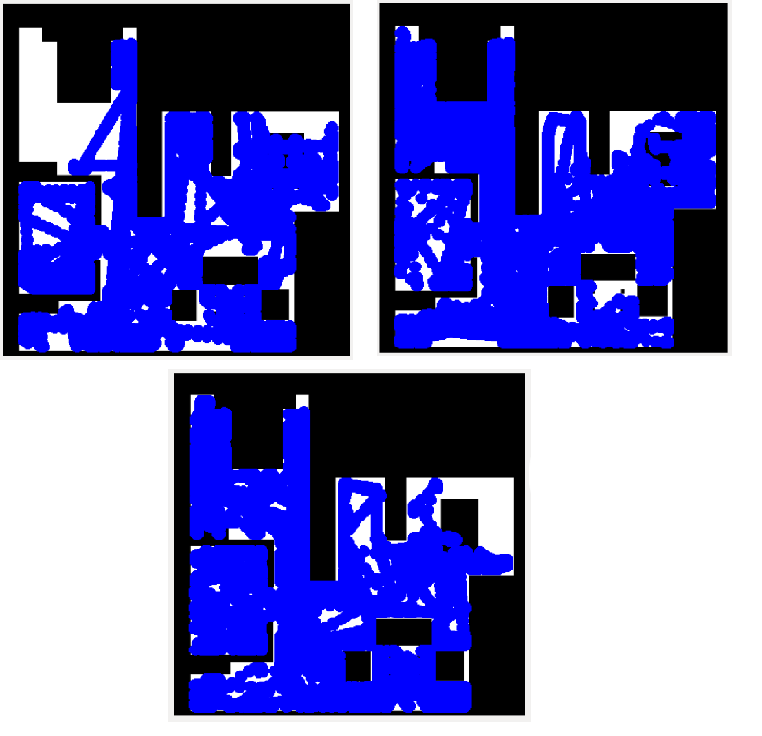
\includegraphics[width=0.7\textwidth]{figures/Vacuum/Referee_hora.png}
		\caption{Superficie recorrida de las pruebas de 90 minutos}
		\label{fig.Referee_hora}
		\end{center}
\end{figure}